
\section{Additional Figures/Tables?}




\begin{figure}[!ht]
    \centering
    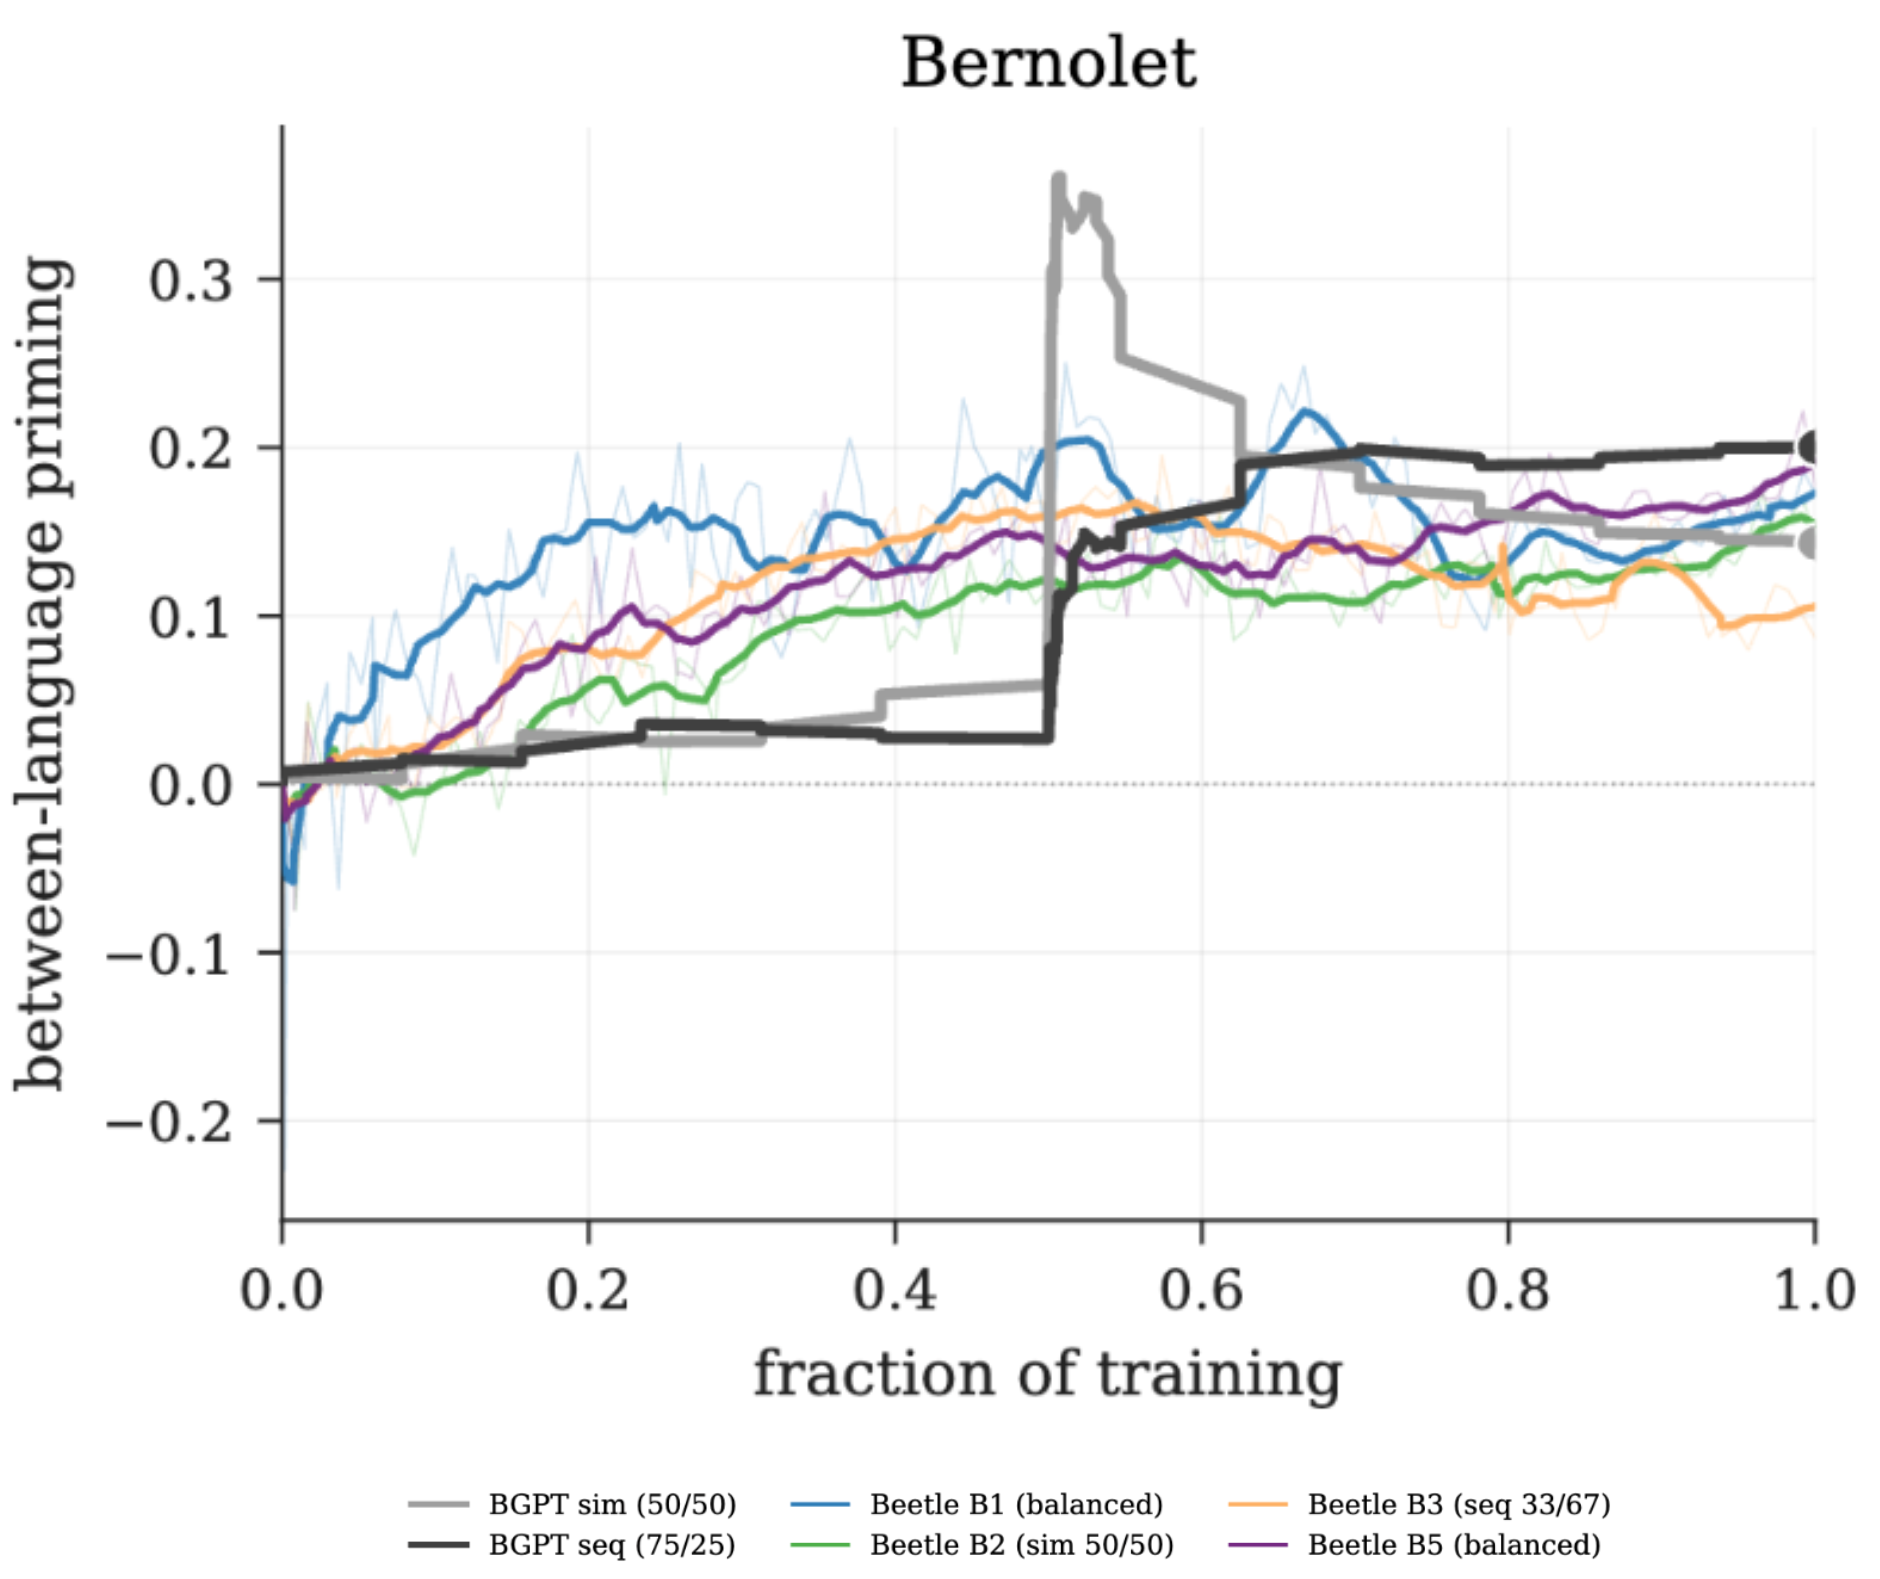
\includegraphics[width=\linewidth]{fig/priming/4.png}
    \caption{[do we want to include this in the main body? basically, BGPT and Beetle get similar structural priming effects for the Dutch-English Bernolet et al (2013) study in \citet{arnett-etal-2025-acquisition}]; probably a good comparison to include to show similar behaviours in BGPT and Beetle? Happy to relegate to appendix otherwise. I have quite a few interesting priming plots for this study, which I would like to include in EMNLP as a BGPT-Beetle Comparison, leaving more  analysis to the CL journal paper. \textcolor{red}{[catherine: i would actually recommend not including anything about structural priming. most people don't know about it and it requires a lot of explanation for people to get. i think you should move all the priming results to the CL doc (or even yet another paper tbh)]}}
    \label{fig:placeholder}
\end{figure}


\begin{figure}
    \centering
    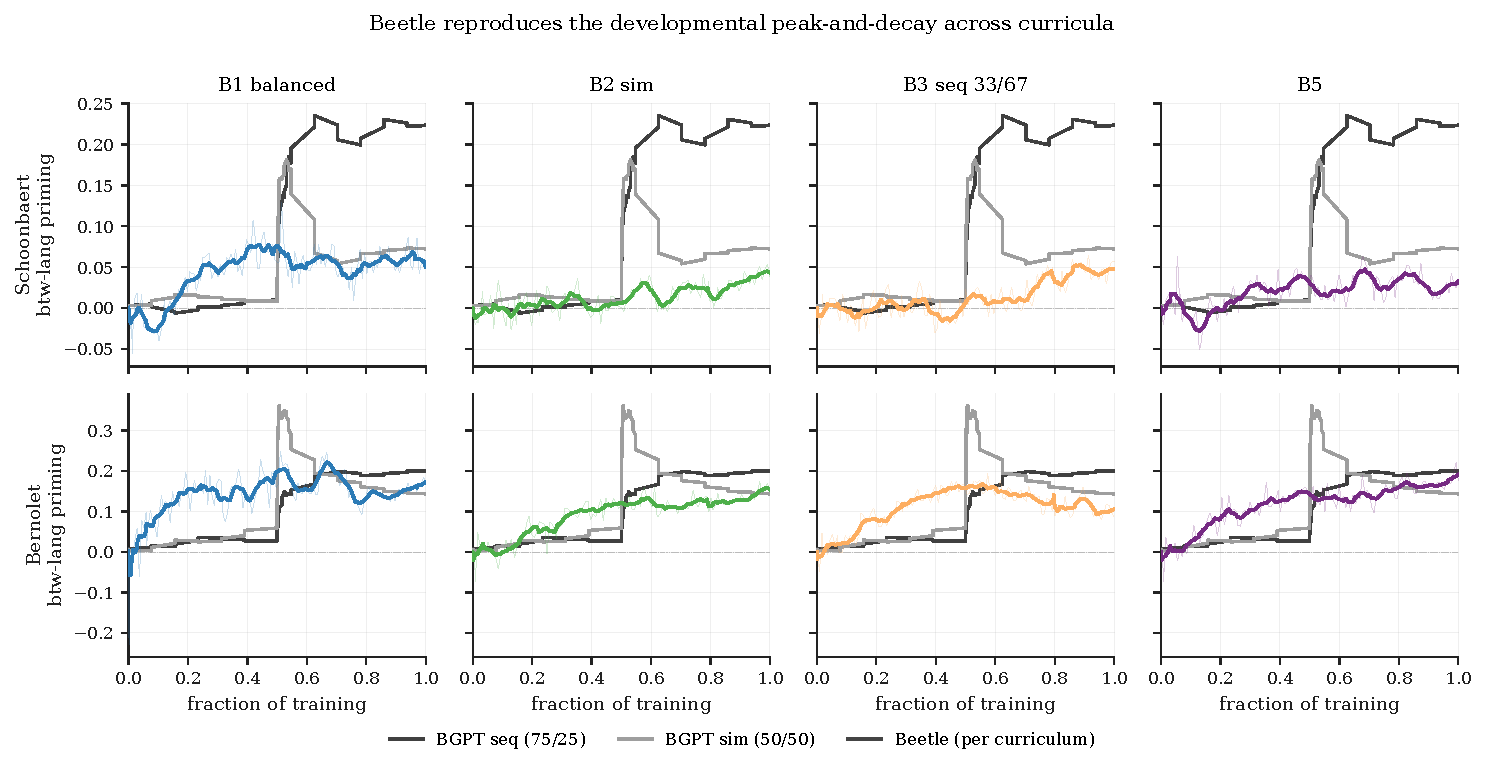
\includegraphics[width=\linewidth]{fig/priming/fig2_trajectory_per_curriculum.pdf}
    \caption{This is an alternative priming fig?}
    \label{fig:placeholder}
\end{figure}

Here are some other tables: 

\begin{table}[!ht]
\small
\setlength{\tabcolsep}{4pt}
\begin{tabular}{lcc}
\toprule
Curriculum & FLORES PPL & MECO $\Delta\log L$ \\
(nld--eng HS) & (eng) $\downarrow$ & (Dutch) $\uparrow$ \\
\midrule
B1 balanced     & \textbf{412}  & 62.33 \\
B4 classroom    & 806           & 121.77 \\
B5 late-onset   & 987           & 137.74 \\
B3-33 sequential& 1033          & \textbf{139.58} \\
B2 simultaneous & 1129          & 135.14 \\
\midrule
mono-eng HS     & 781           & 65.13 \\
\bottomrule
\end{tabular}
\caption{\textcolor{red}{[catherine: the flores ppl column is interesting(well i guess we need the NLL results). this basically shows that training on half the amount of data (B1) leads to better PPL than training only on English? that seems v surprising]}}
\end{table}

\begin{table*}[!ht]
\small
\centering
\begin{tabular}{lccccccc}
\hline
Strategy & BLiMP-en (\%) & BLiMP-nl (\%) & BLiSS RP@0 & BLiSS RP@$\tau$ & BLiSS NGS & BLiSS CPS & MECO \\
\hline
base& 63.86 & 63.51 & 55.96 & 48.35 & 55.88 & 49.49 & 5.135 \\
ewc & 63.83 & 63.37 & 56.64 & 48.58 & 56.02 & 50.62 & 5.136 \\
lamol & 64.46 & 63.24 & 54.60 & 48.81 & 55.47 & 50.06 & 5.143 \\
pre-pretrain & 65.77 & 61.28 & 57.66 & 49.72 & 55.93 & 47.79 & 4.989 \\
alibi & 66.43 & 61.59 & 56.19 & 49.83 & 55.72 & 49.94 & 5.060 \\
\hline
\end{tabular}
\caption{Performance comparison across different training strategies.}
\label{tab:strategy_results}
\end{table*}





\begin{table*}[!ht]
  \centering \small
  \setlength{\tabcolsep}{5pt}
%  \caption{\textbf{Matched-L1 \beetle{} curriculum sweep on MECO~L2 $\Delta\log L$, by training scale.} Each cell is the L1$\to$English model evaluated on the matching L2 reader population (Dutch \texttt{du} / German \texttt{ge} / Chinese \texttt{ch\_s}); larger $\Delta\log L$ indicates better surprisal--reading-time alignment. Scales: 100M (\textsc{HumanScale}, BabyBabelLM); 2B and 24B (\textsc{FineWeb}: FineWeb-2 for L1, FineWeb-Edu for English). \textbf{Bold} marks the best curriculum within each (language, scale) column. The staged-over-balanced advantage holds at all three scales for Dutch and---except 2B B5---for German, but not for Chinese, where balanced (B1) is competitive at every scale (consistent with the L1-dependence discussed in the text). \emph{24B provenance:} Dutch and the German B1/B2 cells are from the original FineWeb release; the German B3/B4/B5 cells and all Chinese cells are from the FineWeb-2 24B release (which supplies a single-source 24B triplet only for Chinese).}
  \label{tab:meco_curriculum_matched}
  \begin{tabular}{l ccc ccc ccc}
    \toprule
    & \multicolumn{3}{c}{\textbf{Dutch} (\texttt{du})} & \multicolumn{3}{c}{\textbf{German} (\texttt{ge})} & \multicolumn{3}{c}{\textbf{Chinese} (\texttt{ch\_s})} \\
    \cmidrule(lr){2-4}\cmidrule(lr){5-7}\cmidrule(lr){8-10}
    Curriculum & 100M & 2B & 24B & 100M & 2B & 24B & 100M & 2B & 24B \\
    \midrule
    B1 balanced       & 62  & 31 & 47          & 75  & 85          & 125          & 106          & \textbf{156} & 168 \\
    B2 simultaneous   & 135 & 34 & \textbf{96} & 166 & 86 & \textbf{185} & 100          & 149          & 160 \\
    B3-33 sequential  & \textbf{140} & \textbf{42} & 75 & \textbf{177} & \textbf{101} & 168 & 103          & 133          & 148 \\
    B4 classroom-20   & 122 & 36 & 55          & 141 & 70          & 177          & 99           & 110          & \textbf{189} \\
    B5 late-onset     & 138 & 40 & 81          & 168 & 78          & 181          & \textbf{115} & 143          & 169 \\
    \bottomrule
  \end{tabular}
  \caption{\textcolor{red}{[catherine: i think this table might be more informative to fig 3 (right)/fig 4/or fig 5, especially if you add more langs..]}}
\end{table*}
